%%\documentclass{article}
%%\standaloneconfig{border=1cm 1cm 1cm 1cm} 
%%\usepackage{pgfplots,calc}
%%\begin{document}
%%\setcounter{figure}{2}
%%\begin{figure}
%%\begin{center}	
%
%\begin{tikzpicture}
%
%\begin{axis}[%
%width=0.7\textwidth,
%height=0.5\textwidth,
%xmode = log,
%ymode = log,
%scale only axis,
%thick,
%xmin=0.1,
%xmax=500,
%xlabel={Depth of Pacinian Corpuscles, DPC (mm)},
%ymin=0,
%ymax=2000,
%grid=major,
%grid style={line width=.1pt, draw=gray!10},
%major grid style={line width=.2pt,draw=gray!50},
%ylabel={Wavelength of Rayleigh wave (mm)},
%axis background/.style={fill=none},
%legend style={legend cell align=left,align=left,font=\scriptsize},
%legend pos = south east,
%legend columns=2
%% legend style={at={(0.98,0.66)}}
%]
%\addplot [color=brown,only marks,mark=o,mark options={solid,thick},mark size=3pt]
%  table[row sep=crcr]{
%1.5	4.40003911713975\\
%3.1	7.63762615825973\\
%1.3	3.16227766016838\\
% };
%\addlegendentry{Human}
%
% \addplot [color=green!40!black,only marks,mark=o,mark options={solid,thick},mark size=3pt]
%  table[row sep=crcr]{
%3.9	9.57427107756339\\
%2	5.24404424085076\\
%25	70.7106781186548\\
%33	86.6025403784439\\
% };
%\addlegendentry{Terrestrial}
%
%% \addplot [color=green!40!black,only marks,mark=square,opacity=0.3,mark options={solid,thick},forget plot,mark size=3pt]
%%  table[row sep=crcr]{
%%2.1	38.7298334620741\\
%% };
%% \node at (axis cs:2.1,38.7298334620741) {\color{green!40!black}\tiny 1};
%%\addlegendentry{Armadillo}
%
% \addplot [color=green!40!black,only marks,mark=square,opacity=0.3,mark options={solid,thick},forget plot,mark size=3pt]
%  table[row sep=crcr]{
%18.6	76.3762615825974\\
% };
%%\addlegendentry{Giraffe}
% \node at (axis cs:18.6,76.3762615825974) {\color{green!40!black}\tiny 1};
%
%\addplot [color=cyan!70!black,only marks,mark=o,mark options={solid,thick},mark size=3pt]
%  table[row sep=crcr]{
%2.8	7.07106781186548\\
% };
%\addlegendentry{Semi-aquatic}
%
%\addplot [color=cyan!70!black,only marks,mark=square,opacity=0.3,mark options={solid,thick},mark size=3pt,forget plot]
%  table[row sep=crcr]{
%3	7.07106781186548\\
% };
%%\addlegendentry{Semi-aquatic}
%
%\addplot [color=blue,only marks,mark=o,mark options={solid,thick},mark size=3pt]
%  table[row sep=crcr]{
%350	1080.12344973464\\
% };
%\addlegendentry{Aquatic}
%
%\addplot [color=blue,only marks,mark=square,opacity=0.3,mark options={solid,thick},mark size=3pt,forget plot]
%  table[row sep=crcr]{
%15	31.6227766016838\\
%%22.4	12.9099444873581\\
% };
%%\addlegendentry{Aquatic}
%%\node at (axis cs:22.4, 12.9099444873581) {\color{blue}\tiny 3};
%
%\addplot [color=red,only marks,mark=square,opacity=0.3,mark options={solid,thick},mark size=3pt]
%  table[row sep=crcr]{
%0.2	3.0276503540975\\
%0.4	10\\
%0.4	4.91596040125088\\
%0.9	7.63762615825973\\
% };
%\addlegendentry{Rodent}
%
%
%\addplot[domain=0.1:1100, dashed,black!70] {2.5327*x};
%\addlegendentry{$y = 2.5x$}
%
%\end{axis}
%\end{tikzpicture}%
%%\end{center}
%%\caption{Squares incomplete data/model, circles complete. Human is for different parts of body. Rodents may be higher because... 1. Giraffe, Hypervasculated skin}
%%\end{figure}
%%
%%
%%\end{document}





%\documentclass{article}
%\standaloneconfig{border=1cm 1cm 1cm 1cm} 
%\usepackage{pgfplots,calc}
%\begin{document}
%\setcounter{figure}{2}
%\begin{figure}
%\begin{center}	

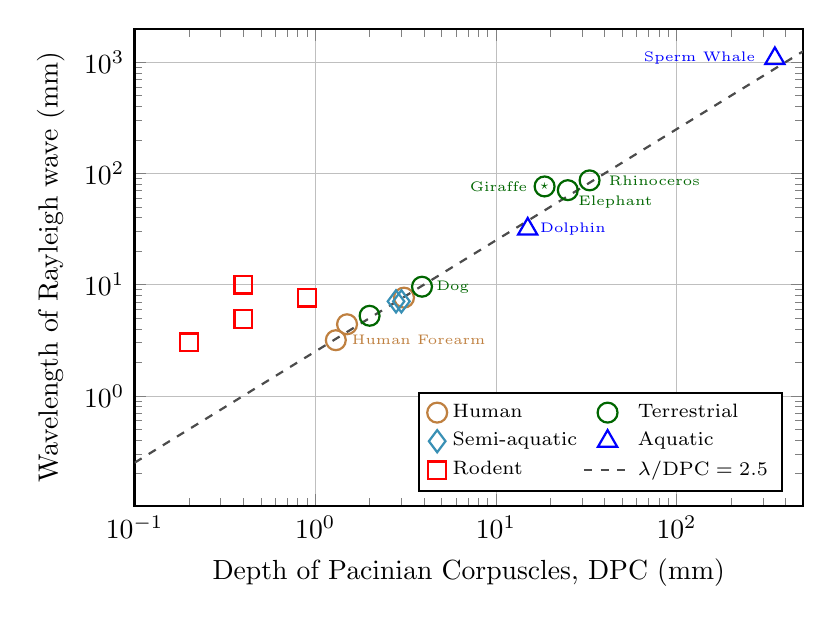
\begin{tikzpicture}

\begin{axis}[%
width=0.7\textwidth,
height=0.5\textwidth,
xmode = log,
ymode = log,
scale only axis,
thick,
xmin=0.1,
xmax=500,
xlabel={Depth of Pacinian Corpuscles, DPC (mm)},
ymin=0,
ymax=2000,
grid=major,
grid style={line width=.1pt, draw=gray!10},
major grid style={line width=.2pt,draw=gray!50},
ylabel={Wavelength of Rayleigh wave (mm)},
axis background/.style={fill=none},
legend style={legend cell align=left,align=left,font=\scriptsize},
legend pos = south east,
legend columns=2
% legend style={at={(0.98,0.66)}}
]
\addplot [color=brown,only marks,mark=o,mark options={solid,thick},mark size=3.6pt]
  table[row sep=crcr]{
1.5	4.40003911713975\\
3.1	7.63762615825973\\
1.3	3.16227766016838\\
 };
\addlegendentry{Human}
\node[anchor=west] at (axis cs:1.4,3.16227766016838) {\tiny \color{brown} Human Forearm};


 \addplot [color=green!40!black,only marks,mark=o,mark options={solid,thick},mark size=3.6pt]
  table[row sep=crcr]{
3.9	9.57427107756339\\
2	5.24404424085076\\
25	70.7106781186548\\
33	86.6025403784439\\
 };
\addlegendentry{Terrestrial}
\node[anchor=west] at (axis cs:37,86.6025403784439) {\tiny \color{green!40!black} Rhinoceros};
\node[anchor=west] at (axis cs:25.1,55) {\tiny \color{green!40!black} Elephant};
\node[anchor=west] at (axis cs:4.1,9.57427107756339) {\tiny \color{green!40!black} Dog};

% \addplot [color=green!40!black,only marks,mark=square,opacity=0.3,mark options={solid,thick},forget plot,mark size=3pt]
%  table[row sep=crcr]{
%2.1	38.7298334620741\\
% };
% \node at (axis cs:2.1,38.7298334620741) {\color{green!40!black}\tiny 1};
%\addlegendentry{Armadillo}

 \addplot [color=green!40!black,only marks,mark=o,opacity=1,mark options={solid,thick},forget plot,mark size=3.6pt]
  table[row sep=crcr]{
18.6	76.3762615825974\\
 };
%\addlegendentry{Giraffe}
\node at (axis cs:18.6,76.3762615825974) {\color{green!40!black}\tiny $\star$};
\node[anchor=east] at (axis cs:17,76.3762615825974) {\color{green!40!black}\tiny Giraffe};

\addplot [color=cyan!70!black,only marks,mark=diamond,mark options={solid,thick},mark size=4pt]
  table[row sep=crcr]{
2.8	7.07106781186548\\
 };
\addlegendentry{Semi-aquatic}

\addplot [color=cyan!70!black,only marks,mark=diamond,opacity=1,mark options={solid,thick},mark size=4pt,forget plot]
  table[row sep=crcr]{
3	7.07106781186548\\
 };
%\addlegendentry{Semi-aquatic}

\addplot [color=blue,only marks,mark=triangle,mark options={solid,thick},mark size=4pt]
  table[row sep=crcr]{
350	1080.12344973464\\
 };
\addlegendentry{Aquatic}
\node[anchor=east] at (axis cs:310,1080.12344973464) {\tiny \color{blue} Sperm Whale};

\addplot [color=blue,only marks,mark=triangle,opacity=1,mark options={solid,thick},mark size=4pt,forget plot]
  table[row sep=crcr]{
15	31.6227766016838\\
%22.4	12.9099444873581\\
 };
\node[anchor=west] at (axis cs:15.4,31.6227766016838) {\tiny \color{blue} Dolphin};

%\addlegendentry{Aquatic}
%\node at (axis cs:22.4, 12.9099444873581) {\color{blue}\tiny 3};

\addplot [color=red,only marks,mark=square,opacity=1,mark options={solid,thick},mark size=3.2pt]
  table[row sep=crcr]{
0.2	3.0276503540975\\
0.4	10\\
0.4	4.91596040125088\\
0.9	7.63762615825973\\
 };
\addlegendentry{Rodent}


\addplot[domain=0.1:1100, dashed,black!70] {2.5*x};
\addlegendentry{$\lambda/\mbox{DPC} = 2.5$}
%\addplot[domain=0.1:1100, dashed,black!70] {1.25*x};
%\addlegendentry{$y = 1.25x$}

\end{axis}
\end{tikzpicture}%





